\documentclass[a4paper, 14pt]{extarticle}

% file's preambule

% Если вы работаете не в XeLaTeX, то сами разбирайтесь =)

% connect packages
%%%%%%%%%%%%%%%%%%%%%%%%%%%%%%%%%%%%%%%%%%%%%%%%%%%%%%%%%%%%%%%%%%%%%%
%\usepackage[T2A]{fontenc}                   %!? закрепляет внутреннюю кодировку LaTeX
%\usepackage[utf8]{inputenc}                 %!  закрепляет кодировку utf8
\usepackage{fontspec}                        % Шрифты
\usepackage{indentfirst}                    %   добавить indent перед первым параграфом
\setlength{\parindent}{1.27cm}
\usepackage{polyglossia}                     % Русский язык
\setdefaultlanguage{russian}
\setmainfont[Ligatures=TeX]{Times New Roman}
\newfontfamily\cyrillicfont{Times New Roman}[Script=Cyrillic]
%\usepackage[english,russian]{babel}         %!  подключает русский и английский
\usepackage{amsmath}                        %!  |
\usepackage{amssymb,textcomp, esvect,esint} %!  |важно для формул 
\usepackage{geometry}                       %!  отступ от граней
\geometry{verbose,a4paper,tmargin=2cm,bmargin=2cm,lmargin=3cm,rmargin=1cm}
\usepackage{amsfonts}                       %!  математические шрифты
\usepackage{amsthm}                         %!  newtheorem и их сквозная нумерация
\usepackage{graphicx}                       %?  графическое изменение текста
\usepackage{soulutf8}% Поддержка переносоустойчивых подчёркиваний и зачёркиваний
\usepackage{enumitem}                       %!  задание макета перечня.
%\usepackage[unicode, pdftex]{hyperref}      %!  оглавление для панели навигации по PDF-документу + гиперссылки
\usepackage{setspace}                       % Межстроковые интервалы
\onehalfspacing
\usepackage{booktabs}                       %!  добавляет книжные линии в таблицы
%\usepackage{hypcap}                         %?  адресация на картинку, а не на подпись к ней
\usepackage{abraces}                        %?  фигурные скобки сверху или снизу текста
\usepackage{caption}                        %-  позволяет корректировать caption 
\DeclareCaptionLabelSeparator{dash}{ - }
\captionsetup[table]{labelformat=simple, labelsep=dash, justification=raggedleft,
singlelinecheck=off}
\captionsetup[figure]{labelformat=simple, labelsep=dash}
\usepackage{multirow}                       %   объединение ячеек в таблицах
\usepackage{longtable}
\usepackage{pifont}                         %!  нужен для крестика
\usepackage{cancel}                         %!  аутентичное перечеркивание текста
\usepackage{ulem}                           %!  перечеркивание текста
\usepackage{tikz}                           %!  высокоуровневые рисунки (кружочек)
\usepackage{titling}                        %-  автоматическое заглавие 
\usepackage{titlesec}  % нормальные заголовки секций
\titleformat{\section}
{\normalfont\large\bfseries\filcenter}{}{1em}{}
\titleformat{\subsection}
  {\normalfont\normalsize\bfseries}{\thesubsection.}{5pt}{}
\titleformat{\subsubsection}
  {\normalfont\normalsize\bfseries}{\thesubsubsection.}{5pt}{}
\titleformat{\paragraph}
  {\normalfont\normalsize\bfseries}{\theparagraph}{5pt}{}

\usepackage{ragged2e} % Для выравнивания текста по ширине
\justifying

%\renewcommand{\thesubsubsection}{\alph{subsubsection}}
\usepackage{blindtext}                      %-  слепой текст
\usepackage{fancyhdr}                       %   добавить верхний и нижний колонтитул
\usepackage{mathptmx}

\usepackage{import}                         %|
\usepackage{xifthen}                        %|
\usepackage{pdfpages}                       %|
%\usepackage{transparent}                    %| вставка ink figures
\usepackage{rotating}
\usepackage{array} % Картиночки в таблицы
%%%%%%%% Алгоритмы
\usepackage{float}
\usepackage{algorithm}
\usepackage{algpseudocode}
%%%%%%%%%%%%%%%

\usepackage{listings} % Для языков программирования 
\usepackage{xcolor}
\lstset {
    language=C++,
    backgroundcolor=\color{black!5}, % set backgroundcolor
    basicstyle=\footnotesize,% basic font setting
}

\usepackage{lmodern}

\colorlet{comment}{green!50!black}
\colorlet{cppcomment}{teal}
\colorlet{symb}{blue!50!black}
\colorlet{number}{violet}

\newcommand*{\textcolorsymb}{\textcolor{symb}}

\definecolor{backcolour}{rgb}{0.95,0.95,0.92}
\definecolor{black_red}{rgb}{0.54, 0, 0}

\lstdefinestyle{cpp}{%
  language=C++,
  columns=flexible,
  basewidth=.5em,  
  tabsize=2,
  basicstyle=\footnotesize,
  backgroundcolor=\color{backcolour},
  showspaces=false,
  showstringspaces=false,
  commentstyle={\itshape\color{comment}\let\textcolorsymb\relax},
  keywordstyle=\bfseries\color{black_red},
  morecomment={[l][\itshape\color{cppcomment}\let\textcolorsymb\relax]//},
  literate=%
    {\{}{\textcolorsymb{\{}}1
    {\}}{\textcolorsymb{\}}}1
    {(}{\textcolorsymb{(}}1
    {)}{\textcolorsymb{)}}1
    {;}{\textcolorsymb{;}}1
    {=}{\textcolorsymb{=}}1
    {<}{\textcolorsymb{<}}1
    {>}{\textcolorsymb{>}}1
    {!}{\textcolorsymb{!}}1
    {\&}{\textcolorsymb{\&}}1 
    {|}{\textcolorsymb{|}}1
    {?}{\textcolorsymb{?}}1
    {:}{\textcolorsymb{:}}1
    {+}{\textcolorsymb{+}}1
    {-}{\textcolorsymb{-}}1
    {,}{\textcolorsymb{,}}1
    {\%}{\textcolorsymb{\%}}1
    {\^}{\textcolorsymb{\textasciicircum}}1
    {~}{\textcolorsymb{\textasciitilde}}1
    %% {/}{\textcolorsymb{/}}1
    %% {*}{\textcolorsymb{*}}1
    % 2 (optionally)
    {==}{\textcolorsymb{==}}2
    {>=}{\textcolorsymb{=>}}2
    {<=}{\textcolorsymb{<=}}2
    {!=}{\textcolorsymb{!=}}2
    {+=}{\textcolorsymb{+=}}2
    {-=}{\textcolorsymb{-=}}2
    {*=}{\textcolorsymb{*=}}2
    {/=}{\textcolorsymb{/=}}2
    {\%=}{\textcolorsymb{\%=}}2
    {\&\&}{\textcolorsymb{\&\&}}2
    {||}{\textcolorsymb{||}}2
    {++}{\textcolorsymb{++}}2
    {--}{\textcolorsymb{--}}2
    {>>}{\textcolorsymb{>\kern0pt>}}2
    {<<}{\textcolorsymb{<\kern0pt<}}2
    {::}{\textcolorsymb{::}}2
    % 3 (optionally)
    {>>=}{\textcolorsymb{>\kern0pt>=}}3
    {<<=}{\textcolorsymb{<\kern0pt<=}}3
    % Remove byte order mark
    {^^ef^^bb^^bf}{}0
}
\lstnewenvironment{cpp}{\lstset{style=cpp}}{}
\lstset{style=cpp}
  


%%%%%%%%%%%%%%%%%%%%%%%%%%%%%%%%%%%%%%%%%%%%%%%%%%%%%%%%%%%%%%%%%%%%%%


%%%%%%%%%%%%%%%%%% ВСТАВКА РИСУНКО ИЗ INKSCAPE %%%%%%%%%%%%%%%%%%%%%%%
\newcommand{\incfig}[1]{%
    \def\svgwidth{\columnwidth}
    \import{./figures/}{#1.pdf_tex}
}

%%%%%%%%%%%%%%%%%%%%%%%%%%%%%%%%%%%%%%%%%%%%%%%%%%%%%%%%%%%%%%%%%%%%%%


\newenvironment{itemize*}
{
    \begin{itemize}
        \setlength{\itemsep}{1pt}
        \setlength{\parskip}{1pt}}
    {\end{itemize}
}

\newenvironment{enumerate*}
{
    \begin{enumerate}
        \setlength{\itemsep}{1pt}
        \setlength{\parskip}{1pt}}
    {\end{enumerate}
}

%%%%%%%%%%%%%%%%%%%%%%%%%%%%%%%%%%%%%%%%%%%%%%%%%%%%%%%%%%%%%%%%%%%%%%


\begin{document}

\includepdf{titul_sixth}
\newpage
\tableofcontents
\newpage
\section{Ответы на вопросы}
\begin{enumerate}
  \item Существует три уровня представления данных: уровень пользователя (предметная область),
    логический и физический.

Каждый объект предметной области характеризуется своими атрибутами,
каждый атрибут имеет имя и значение. 

Логический (концептуальный) уровень - это абстрактное представление
(абстрактный уровень) данных, независимое от представления в ЭВМ.

Физический уровень - это практическая реализация базы данных на том или ином
носителе в ЭВМ. Сюда входят и программные средства управления этими носителями.
\item Тип данных определяет то, чем именно представляются данные, операции над ними, а также способы
хранения значений типа.
\item Структура данных определяет множество связей между ними, а также способ их организации.
\item Структура данных — программная единица, позволяющая хранить и обрабатывать
  множество однотипных или логически связанных данных в вычислительной технике.
  Для добавления, поиска, изменения и удаления данных структура данных
  предоставляет некоторый набор функций, составляющих её интерфейс.
\item Линейная структура данных - это такая структура данных, в которой
  операции осуществляются линейно. ps: https://askinglot.com/what-is-linear-data-structure-explain-with-example
\item Линейный однонаправленный список — это структура данных, состоящая из элементов
одного типа, связанных между собой последовательно посредством указателей.
\item Стек - это линейная структура данных, в которой операции получения и удаления
  элемента структуры осуществляется в определенном порядке LIFO - новый элемент
  стека становится последним и он же становится следующим удаляемым.
  Позиция данного элемента называется вершиной стека.
\item Очередь - это линейная структура данных, в которой операции получения и удаления
  элемента структуры осуществляется в определенном порядке FIFO - новый элемент
  стека становится последним, первый добавленный элемент является следующим
  удаляемым.
\item Стек может быть построен на списке, но список не всегда будет стеком
  т.к. в стеке соблюдается специальный порядок обработки данных LIFO
  (был рассмотрен выше).
\item Двунаправленный список
\item Сложность вставки в произвольную позицию массива размера n равна $O(n)$
  т.к. сама вставка занимает $O(1)$ + сдвиг элементов массива в худшем
  случае  $O(n)$.

  Сложность вставки в произвольную позицию списка происходит за
  $O(1)$ + получение адреса элемента списка в худшем случае  $O(n)$.
  Отсюда сложность  $O(n)$.
\item Удаление элемента из массива и из списка имеет аналогичное вставке
  поведение, т.е. сложность  $O(n)$. 
\item Трюк Вирта заключается в проходе списка при помощи одного
указателя. Можно хранить XOR двух указателей, на предыдущий
элемент списка и на следующий, таким образом имея оба под рукой в
одном указателе. %
\item template<typename T> class Node {T value; Node* next;};
\item Приведен ниже в отчете главного задания.
\item Код предоставлен таккже в отчете главного задания. 
\item В этом коде лишней является ветка условного оператора
  с проверкой на нулевой указатель т.к. при обращении по нулевому указателю
  произойдет ошибка программы. Код вставляет новый узел в последующий после
  LL узел.
\end{enumerate}

\section{Главное задание}
\subsection{Постановка задачи}
Требуется реализовать программу решения следующих задач варианта
No9 по использованию линейного однонаправленного списка:
\begin{enumerate}
  \item Информационная часть узла содержит символы, которые формируют "слова",
    разделенные пробелом.
  \item Разработать функцию для создания исходного списка, используя
функцию вставки нового узла перед первым узлом.
\item Разработать функцию вывода списка.
\item Разработать функцию, которая находит последнее слово и переставляет его в начало списка.
\item Разработать функцию, которая удаляет второе слово.
\item Разработать функцию, которая заменяет k-ое слово на новое слово. Длина нового слова
может быть больше длины k-ого слова.
\item В основной программе выполнить тестирование каждой функции.
\end{enumerate}
\subsection{Определение операций над списком}
\paragraph{Структура узла линейного списка}
Согласно варианту No9 в качестве информационной части узла списка
используются символы. Класс узла хранит в себе значение данного узла
и указатель на следующий элемент в списке. Сам список хранит в себе
корень списка, через который происходит доступ к остальным узлам списка,
а также размер данного списка (количество узлов).

\begin{figure}[htpb]
  \centering
  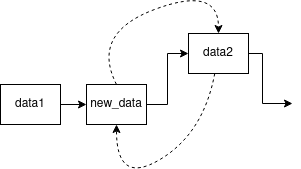
\includegraphics[width=0.5\textwidth]{pictures/insert_before.png}
  \caption{Изображение вставки узла перед элементом (перед data2)}
  \label{fig:insert_before}
\end{figure}

\begin{figure}[htpb]
  \centering
  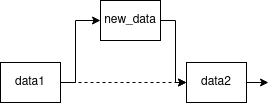
\includegraphics[width=0.5\textwidth]{pictures/insert_after.png}
  \caption{Изображение вставки узла после элемента (после data1)}
  \label{fig:insert_after}
\end{figure}

\begin{figure}[htpb]
  \centering
  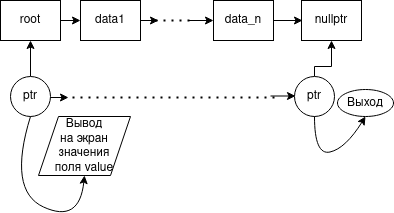
\includegraphics[width=0.5\textwidth]{pictures/print_list.png}
  \caption{Алгоритм вывода элементов списка}
  \label{fig:print_list}
\end{figure}

\begin{figure}[htpb]
  \centering
  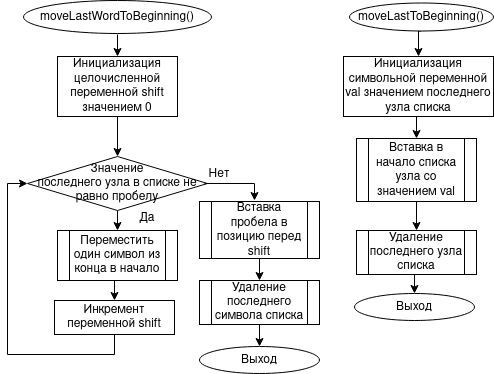
\includegraphics[width=0.7\textwidth]{pictures/moveLastWordToBeginning.png}
  \caption{Алгоритм переставления слова в начало списка}
  \label{fig:move_beginning}
\end{figure}

\begin{figure}[htpb]
  \centering
  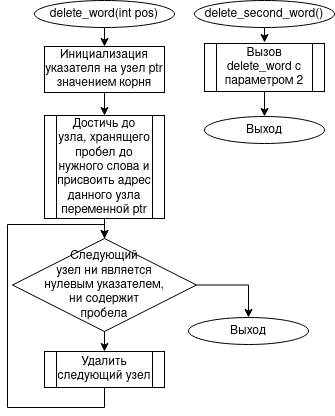
\includegraphics[width=0.5\textwidth]{pictures/deleteSecondWord.png}
  \caption{Алгоритм удаления второго слова}
  \label{fig:delete_second}
\end{figure}

\begin{figure}[htpb]
  \centering
  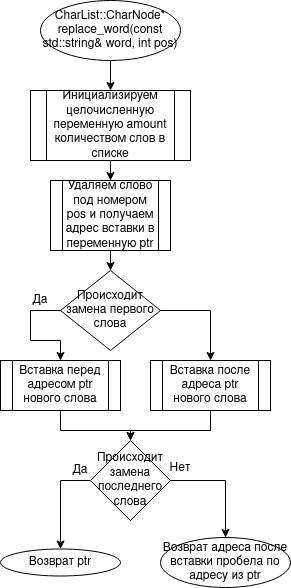
\includegraphics[width=0.5\textwidth]{pictures/replace_word.png}
  \caption{Алгоритм замены любого слова в списке}
  \label{fig:replace_word}
\end{figure}

\newpage
\subsection{Код программы}
Реализация на C++:

\textit{Код файла charlist.h}
\lstinputlisting{code/charlist.h}

\textit{Код файла charlist.cpp}
\lstinputlisting{code/charlist.cpp}

\textit{Код файла list\_lin.cpp}
\lstinputlisting{code/lin_list.cpp}
\newpage
\subsection{Результаты тестирования}
\begin{figure}[htpb]
  \centering
  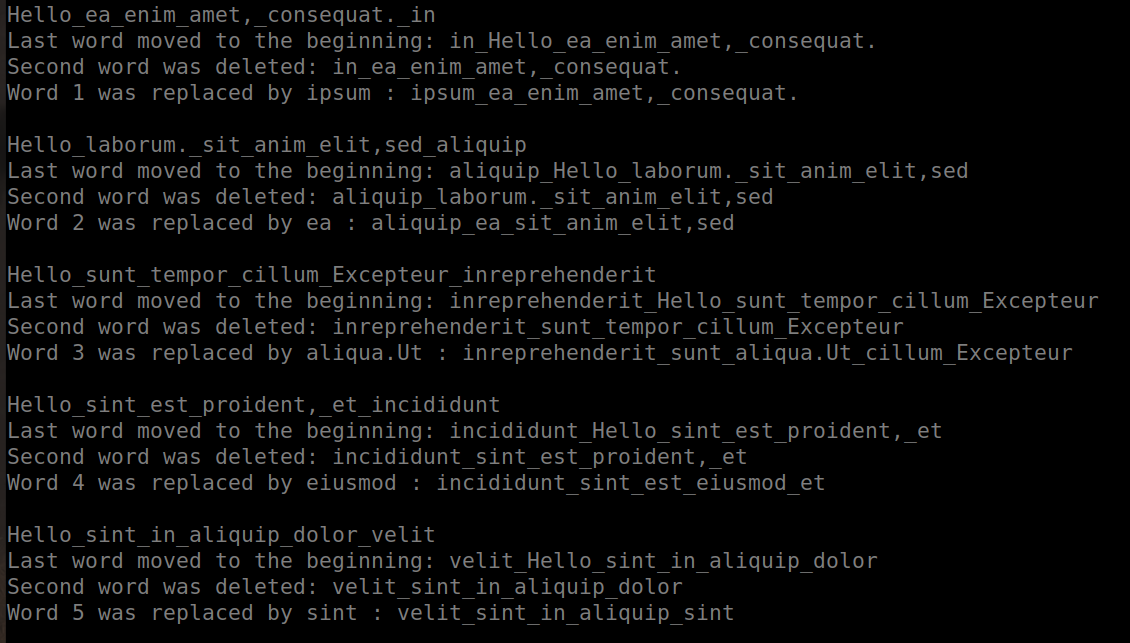
\includegraphics[width=1\textwidth]{pictures/test_list.png}
  \caption{Результаты тестирования программы}
  \label{fig:test}
\end{figure}
\newpage
\section*{Выводы}
\addcontentsline{toc}{section}{Выводы}
В ходе выполнения работы была реализована структура
«однонаправленный список», поддерживающий следующие обязательные операции: вывод
хранящихся значений узлов списка, добавление элемента перед и после узла, перемещение
последнего слова в начало, удаление второго слова из списка,
замена одного слова списка на другое по позиции в списке. Также в ходе
выполнения работы были усвоены основы работы с односвязными списками.
Тестирование подтвердило правильность работы методов.
\section*{Список информационных источников}
\addcontentsline{toc}{section}{Список информационных источников}
\begin{enumerate}[leftmargin=*] % delete left margin
  \item Thomas H. Cormen, Clifford Stein и другие: Introduction to Algorithms, 3rd Edition.
    Сентябрь 2009. The MIT Press.
  \item N. Wirth: Algorithms and Data Structures. Август 2004.
    \\ https://people.inf.ethz.ch/wirth/AD.pdf.
  \item Linked list~//~Wikipedia \\~
    [Электронный ресурс]. URL:
    \\ https://en.wikipedia.org/wiki/Linked\_list
    (Дата обращения: 30.04.2021)
   \item Курс Algorithms, part 1 // Coursera [Электронный ресурс]. URL:
     \\ https://www.coursera.org/learn/algorithms-part1
     (Дата обращения: 26.04.2021)
\end{enumerate}
\end{document}
